\section{ Model comparisons}\label{model_comparisons}

As mentioned in section \ref{cnn_ref}, we used Keras Tuner model to find hyperparameters that would yield the highest accuracy.
Instead of hard-coding hyperparameters when building a model with Keras API, we defined a search space of possible values with \verb|HyperParameter| class and used that as a hyperparameter.

We passed the created model to a \verb|RandomSearch| class, with few other parameters such as batch size, number of epochs and maximum number of trials.
As we started the hyperparameter search, Keras Tuner started picking a randomly set of hyperparameters, which were used to train a model.
This process was repeated for a trial number of times.
Used hyperparameters and achieved accuracy on validation set for each trained model were logged in a text file for later use.

After training a number of different models we picked a few and compared them.
Comparison of models trained in Edge Impulse Studio was also done.


\subsection{ Hyperparameter search space and results analysis}

General structure of CNN model was already described in section \ref{cnn_ref} and in Figure \ref{model_code}.
We decided to search for the following hyperparameters: 

\begin{itemize}
    \item Number of filters in all three convolutional layers (can be different for each layer)
    \item Size of filters in all three convolutional layers (same for all layers)
    \item Size of dense layer
    \item Dropout rate 
    \item Learning rate
\end{itemize}

Possible values of hyperparameters (also known as hyperparameter search space) are specified in Table \ref{hyper_table1}.
\newline
\begin{table}[ht]
    \centering
    \caption{ First hyperparameter search space}
    \rowcolors{2}{white}{gray!25}
    \begin{tabular}{@{} *5l @{}}    \toprule
        \textbf{Hyperparameter} & \textbf{Set of values}\\\midrule
        \verb|FilterNum1|       & From 16 to 80, with a step of 8\\ 
        \verb|FilterNum2|       & From 16 to 80, with a step of 8\\ 
        \verb|FilterNum3|       & From 16 to 80, with a step of 8\\
        \verb|FilterSize|       & 3 x 3 or 3 x 4\\
        \verb|DenseSize|        & From 16 to 96, with a step of 8\\
        \verb|DropoutRate|      & From 0.2 to 0.5, with a step of 0.05\\
        \verb|LearningRate|     & 0.0001 or 0.0003\\\toprule
        \textbf{Random search}  & \textbf{value}\\
        \textbf{variable}       & \\\midrule
        \verb|EPOCHS|           & 25\\
        \verb|BATCH_SIZE|       & 100\\
        \verb|MAX_TRIALS|       & 300\\\bottomrule
    \end{tabular}
    \label{hyper_table1}
\end{table}

Search space of \verb|FilterNumX|, \verb|DenseSize| and \verb|DropoutRate| hyperparameters was chosen based on initial training tests conducted on thermal image dataset and other various models that were trained on similar data.
Value of \verb|FilterSize| is usually 3 x 3, however most of example ML projects that we could find on the Internet were training on image data of the same dimensions.
We wanted to test how would a filter with same ratio of dimensions as image data (3 x 4 and 60 x 80 respectively) perform.
Hyperparameter \verb|learning_rate| was chosen heuristically, we saw that 10 times higher values, such as 0.001 or 0.003, would leave model's accuracy stuck at suboptimal optima, from where it could not be improve anymore.

We also had to set 3 variables that directly affected how long will random search last.
From initial tests we saw that models usually reached maximum possible accuracy around \nth{20} epoch, to give some headroom we set the number of epochs to 25.
We kept batch size relatively small, at 100, which meant that weights would get updated regularly.
Hyperparameter \verb|MAX_TRIALS| had the biggest impact on the training time, we set it to 300.

Training lasted for about 12 hours. 
After it was done we compiled a list of all 300 trained models and their different hyperparameter values, number of parameters and achieved accuracies
Part of it can be seen in Table \ref{hyper_results1}.
\newline
\begin{table}[ht]
    \centering
    \caption{ Partial results of first random search of hyperparameters}
    \rowcolors{2}{gray!25}{white}
    \begin{tabular}{llllllllrl}
    \textbf{Model ID} & \rot{FilterNum1} & \rot{FilterNum2} & \rot{FilterNum3} & \rot{DenseSize} & \rot{DropoutRate}  &\rot{FilterSize} & \rot{LearningRate} & \rotatebox{45}{\parbox{2cm}{Number of parameters}} & \rot{Accuracy[\%]}  \\\toprule
        0a & 72 & 80 & 64 & 72 & 0.4  & 3x4 & 0.0003 & 1,514,400 & 98.35\\
        1a & 32 & 40 & 72 & 56 & 0.35 & 3x4 & 0.0001 & 1,260,332 & 98.31\\
        2a & 40 & 48 & 32 & 64 & 0.35 & 3x4 & 0.0001 &   656,797 & 98.31\\
        3a & 56 & 16 & 48 & 72 & 0.4  & 3x4 & 0.0001 & 1,057,924 & 98.28\\
        4a & 80 & 64 & 40 & 96 & 0.45 & 3x4 & 0.0003 & 1,245,788 & 98.28\\\midrule
       96a & 16 & 32 & 72 & 80 & 0.25 & 3x4 & 0.0001 & 1,762,508 & 98.00\\
       97a & 72 & 56 & 40 & 56 & 0.45 & 3x4 & 0.0003 &   748,580 & 98.00\\
       98a & 32 & 24 & 24 & 48 & 0.35 & 3x3 & 0.0001 &   358,308 & 98.00\\
       99a & 48 & 16 & 40 & 40 & 0.45 & 3x3 & 0.0003 &   493,412 & 98.00\\
      100a & 24 & 72 & 64 & 40 & 0.45 & 3x3 & 0.0003 &   844,684 & 98.00\\\midrule
      191a & 64 & 56 & 16 & 52 & 0.4  & 3x3 & 0.0001 &   386,996 & 97.76\\
      192a & 48 & 40 & 24 & 24 & 0.4  & 3x4 & 0.0001 &   208,172 & 97.73\\
      193a & 56 & 64 & 72 & 24 & 0.25 & 3x4 & 0.0003 &   617,692 & 97.73\\
      194a & 48 & 72 & 48 & 32 & 0.25 & 3x4 & 0.0003 &   544,652 & 97.73\\\midrule
      295a & 48 & 32 & 64 & 16 & 0.5  & 3x4 & 0.0001 &   351,012 & 95.87\\
      296a & 40 & 24 & 56 & 24 & 0.5  & 3x4 & 0.0001 &   431,572 & 95.77\\
      297a & 56 & 16 & 80 & 16 & 0.2  & 3x4 & 0.0001 &   411,020 & 95.63\\
      298a & 24 & 16 & 48 & 24 & 0.5  & 3x4 & 0.0001 &   359,924 & 94.46\\
      299a & 40 & 48 & 56 & 16 & 0.35 & 3x3 & 0.0003 &   310,860 & 82.86\\\bottomrule
    \end{tabular}
    \label{hyper_results1}
\end{table}

After analyzing results we came to several conclusions:

\begin{enumerate}
    \item We saw that almost all trained models, except of the last one, achieved accuracy above 90 \%. This proved that the general architecture of the model was appropriate for the problem.
    \item We could not see any visible correlation between a specific choice of a certain hyperparameter and accuracy. This showed that selection of hyperparameters is really a non-heuristic task, at least for our particular problem.
    \item Filter of size 3 x 4 did not perform significantly better compared to one with size 3 x 3. 
    \item There is a weak correlation between number of parameters (model's complexity) and accuracy, however, models with small size and great accuracy exist, model \textit{2a} is example of that.
    \item First 200 models cover an accuracy range of 0.62 \%. However inside of this range model number of parameters varies hugely, for example, model \textit{192a} has more than 8 times less parameters than model than model \textit{96a}, although the difference in accuracy (0.27 \%) is negligible.
\end{enumerate}

It is apparent from results that large models are not necessary to achieve high accuracy on our training data, so we decided to run the random search of hyperparameters again.

This time we lowered the maximum and the minimum numbers of filters and size of the dense layer.
We decreased all steps from 8 to 2, thus increasing the number of possible configurations.
We decided to lower the bottom boundary of \verb|DropoutRate| from 0.2 to 0.0, which means that some models will not be using dropout layer at all.
We expected that training without dropout layer would produce suboptimal results, however we wanted to test it.
Redefined search space for second random search can be seen in Table \ref{hyper_table2}
We increased the number of \verb|MAX_TRIALS| from 300 to 500, as we were expecting that more models will end up underfitting and also because there would be more possible options because of smaller step size.
Partial table of results of random hyperparameter search can be seen in Table \ref{hyper_results2}.

\begin{table}[ht]
    \centering
    \caption{ Second hyperparameter search space}
    \rowcolors{2}{white}{gray!25}
    \begin{tabular}{@{} *5l @{}}    \toprule
        \textbf{Hyperparameter} & \textbf{Set of values}\\\midrule
        \verb|FilterNum1|       & From 4 to 48, with a step of 2\\ 
        \verb|FilterNum2|       & From 4 to 48, with a step of 2\\ 
        \verb|FilterNum3|       & From 4 to 48, with a step of 2\\
        \verb|FilterSize|       & 3 x 3 or 3 x 4\\
        \verb|DenseSize|        & From 4 to 48, with a step of 2\\
        \verb|DropoutRate|      & From 0.0 to 0.5, with a step of 0.05\\
        \verb|LearningRate|     & 0.0001 or 0.0003\\\toprule
        \textbf{Random search}  & \textbf{value}\\
        \textbf{variable}       & \\\midrule
        \verb|EPOCHS|           & 25\\
        \verb|BATCH_SIZE|       & 100\\
        \verb|MAX_TRIALS|       & 500\\\bottomrule
    \end{tabular}
    \label{hyper_table2}
\end{table}

\begin{table}[ht]
    \centering
    \caption{ Partial results of second random search of hyperparameters}
    \rowcolors{2}{gray!25}{white}
    \begin{tabular}{llllllllrl}
    \textbf{Model ID} & \rot{FilterNum1} & \rot{FilterNum2} & \rot{FilterNum3} & \rot{DenseSize} & \rot{DropoutRate}  &\rot{FilterSize} & \rot{LearningRate} & \rotatebox{45}{\parbox{2cm}{Number of parameters}} & \rot{Accuracy[\%]}  \\\toprule
        0b & 40 & 20 & 20 & 48 & 0.25 & 3x4 & 0.0001 & 304,216 & 98.14\\
        1b & 44 & 10 & 28 & 42 & 0.2  & 3x4 & 0.0003 & 362,264 & 98.14\\
        2b & 18 & 38 & 26 & 38 & 0.1  & 3x4 & 0.0003 & 316,956 & 98.11\\\midrule
       95b & 20 & 16 & 34 & 40 & 0.3  & 3x3 & 0.0003 & 416,230 & 97.62\\
       96b & 46 & 42 & 28 & 32 & 0.4  & 3x3 & 0.0003 & 297,466 & 97.62\\
       97b & 30 & 26 & 30 & 34 & 0.2  & 3x3 & 0.0001 & 320,570 & 97.59\\\midrule
      195b & 28 & 16 & 40 & 24 & 0.1  & 3x3 & 0.0001 & 298,252 & 97.31\\
      196b & 44 & 30 & 32 & 20 & 0.3  & 3x4 & 0.0003 & 220,098 & 97.31\\
      197b & 46 & 40 & 10 & 40 & 0.1  & 3x3 & 0.0001 & 140,874 & 97.31\\\midrule
      295b & 20 &  8 & 34 & 26 & 0.3  & 3x3 & 0.0003 & 269,464 & 96.90\\
      296b & 18 & 16 & 10 & 20 & 0.3  & 3x4 & 0.0003 &  65,740 & 96.87\\
      297b &  8 & 22 & 28 & 16 & 0.1  & 3x3 & 0.0001 & 141,742 & 96.87\\\midrule
      395b & 10 & 20 & 12 & 30 & 0.0  & 3x3 & 0.0001 & 112,246 & 96.87\\
      396b & 24 & 24 & 46 & 18 & 0.2  & 3x3 & 0.0003 & 263,924 & 96.14\\
      397b &  6 & 18 & 12 & 24 & 0.4  & 3x4 & 0.0001 &  90,520 & 96.11\\\midrule
      497b & 42 & 30 & 22 &  6 & 0.4  & 3x3 & 0.0003 &  57,386 & 82.86\\
      498b &  4 &  4 & 20 & 12 & 0.4  & 3x3 & 0.0003 &  72,992 & 82.86\\
      499b & 32 & 36 & 36 &  4 & 0.15 & 3x3 & 0.0001 &  65,648 & 82.86\\\bottomrule
    \end{tabular}
    \label{hyper_results2}
\end{table}

\clearpage
Some observations:
\begin{enumerate}
    \item We can see that the accuracy of the best model \textit{0b} compared to the best model \textit{0a} from previous search is only 0.21 \% lower, although it has about 5 times less parameters.
    \item Although that it might seem that \verb|FilterSize| of 3 x 4 yields best results, we did not saw a strong tendency towards 3 x 3 or 3 x 4 filter size after manually analyzing best 30 models.
    \item We can see that the worst three models have the same accuracy of 82.86 \%, same as the worst performing model from first random search. There are 82.86 \% images of elephants in validation class, which means that model probably assigned all validation images to elephant class and was satisfied with achieved accuracy.
    \item We can see that the model \textit{296b} has a quite low number of parameters, only 65,740 when compared to it neighbours.
\end{enumerate}


\subsection{ Comparison of selected, re-trained models}
    
Two random searches gave us a large amount of different models to choose from.
In every other ML application where the execution time would not be a constraint, we could simply take the best performing model and be done with it.
In our case we had to make a trade off between model's accuracy and execution speed.

For comparison and later on device performance testing we decided to pick and retrain\footnotemark 6 models: \textit{0a}, \textit{2a}, \textit{0b}, \textit{172b}, \textit{338b} and \textit{460b}, their properties are listed in Table \ref{hyper_selection}.

Chosen models vary greatly in number of parameters.
Models \textit{0a}, \textit{2a}, \textit{0b} have high number of parameters but their accuracy is high.
Models \textit{172b}, \textit{338b} and \textit{460b} were chosen because of their small size and reasonably good accuracy.
\footnotetext{Retraining was required as Keras Tuner module only saved hyperparameter settings during search and not each trained model.
As the weights are initially randomized, accuracy of retrained models is going to be similar but not exact when compared to the accuracy returned by random search.}

\begin{table}[ht]
    \centering
    \caption{ Properties of selected models}
    \rowcolors{2}{gray!25}{white}
    \begin{tabular}{llllllllrl}
    \textbf{Model ID} & \rot{FilterNum1} & \rot{FilterNum2} & \rot{FilterNum3} & \rot{DenseSize} & \rot{DropoutRate}  &\rot{FilterSize} & \rot{LearningRate} & \rotatebox{45}{\parbox{2cm}{Number of parameters}} & \rot{Accuracy[\%]}  \\\toprule
        0a & 72 & 80 & 64 & 72 & 0.4  & 3x4 & 0.0003 & 1,514,400 & 98.35\\
        2a & 40 & 48 & 32 & 64 & 0.35 & 3x4 & 0.0001 &   656,797 & 98.31\\
        0b & 40 & 20 & 20 & 48 & 0.25 & 3x4 & 0.0001 &   304,216 & 98.14\\
      172b & 42 & 44 &  8 & 14 & 0.1  & 3x4 & 0.0001 &    60,672 & 97.38\\
      338b &  4 & 18 &  6 & 10 & 0.05 & 3x4 & 0.0003 &    20,290 & 96.63\\
      460b &  6 & 28 &  4 &  8 & 0.1  & 3x4 & 0.0003 &    13,114 & 93.60\\\bottomrule
    \end{tabular}
    \label{hyper_selection}
\end{table}

As we are dealing with imbalanced dataset, where 82.86 \% of our validation data consists of elephant images, accuracy is not the best metric to use when comparing models.
Simply classifying all images into elephant class would yield accuracy of 82.86 \%, which sounds high, although it would not actually do any classification.

When analysing performance of a model on an imbalanced dataset it is more appropriate to use precision and recall metrics\footnotemark.
They can give us a better idea how well the model is performing on data of specific classes.
Calculated metrics can be seen in Table \ref{precision_recall_table}, we abbreviated precision to PR and recall to RE for clarity.
\footnotetext{Precision tells us what percentage of data points in a specific predicted class actually fall into that class.
Recall tells us what percentage of data points inside a certain class were actually predicted correctly\cite{geron}.}
\begin{table}[ht]
    \caption{ Precision and recall metrics of trained models}
    \rowcolors{2}{gray!25}{white}
    \makebox[\textwidth]{%
    \begin{tabular}{lrrrrrrrrr}\toprule
        \textbf{Model ID}                 & 0a & 2a & 0b & 172b & 338b & 460b\\\toprule
        \textbf{Metrics}                &&&&&\\\toprule
        accuracy[\%]                    & \cellcolor{tbgreen} 98.18     
                                        & \cellcolor{tbgreeny}98.04   
                                        & \cellcolor{tbgreeny}98.04   
                                        & \cellcolor{tbyellow}96.80  
                                        & \cellcolor{tbyellow}96.28  
                                        & \cellcolor{tbred}   93.4 \\

        number of parameters            & \cellcolor{tbred}  1,515K 
                                        & \cellcolor{tbyellow} 657K 
                                        & \cellcolor{tbyellow} 304K 
                                        & \cellcolor{tbyellow}  61K 
                                        & \cellcolor{tbgreeny}  20K 
                                        & \cellcolor{tbgreen}   13K\\\midrule

        PR of elephant class[\%]        & \cellcolor{tbyellow}99.22     
                                        & \cellcolor{tbgreen}99.46   
                                        & \cellcolor{tbyellow}99.25   
                                        & \cellcolor{tbgreeny}99.29  
                                        & \cellcolor{tbyellow}98.80  
                                        & \cellcolor{tbred}97.80\\
        PR of human class[\%]           & \cellcolor{tbgreen}96.92     
                                        & \cellcolor{tbgreeny}95.38   
                                        & \cellcolor{tbgreeny}95.38   
                                        & \cellcolor{tbyellow}92.00  
                                        & \cellcolor{tbyellow}91.69  
                                        & \cellcolor{tbred}80.31\\
        PR of cow class[\%]             & \cellcolor{tbgreeny}90.99     
                                        & \cellcolor{tbgreen}93.69   
                                        & \cellcolor{tbyellow}90.09   
                                        & \cellcolor{tbyellow}84.68  
                                        & \cellcolor{tbyellow}75.68  
                                        & \cellcolor{tbred}69.37\\
        PR of nature/random class[\%]   & \cellcolor{tbgreeny}77.42     
                                        & \cellcolor{tbyellow}64.52   
                                        & \cellcolor{tbgreen}79.03   
                                        & \cellcolor{tbyellow}46.77  
                                        & \cellcolor{tbyellow}59.68 
                                        & \cellcolor{tbred}40.32\\\midrule
        RE of elephant class[\%]        & \cellcolor{tbgreen}99.29     
                                        & \cellcolor{tbyellow}98.80   
                                        & \cellcolor{tbgreeny}98.84   
                                        & \cellcolor{tbyellow}97.87  
                                        & \cellcolor{tbyellow}98.43  
                                        & \cellcolor{tbred}97.39\\
        RE of human class[\%]           & \cellcolor{tbyellow}93.20     
                                        & \cellcolor{tbgreeny}94.51   
                                        & \cellcolor{tbgreen}95.09   
                                        & \cellcolor{tbyellow}91.44  
                                        & \cellcolor{tbyellow}89.22  
                                        & \cellcolor{tbred}85.57\\
        RE of cow class[\%]             & \cellcolor{tbgreeny}94.39     
                                        & \cellcolor{tbyellow}92.04   
                                        & \cellcolor{tbgreen}96.15   
                                        & \cellcolor{tbyellow}89.52  
                                        & \cellcolor{tbyellow}84.00  
                                        & \cellcolor{tbred}81.91\\
        RE of nature/random class[\%]   & \cellcolor{tbyellow}87.27     
                                        & \cellcolor{tbgreen}97.56   
                                        & \cellcolor{tbyellow}84.48   
                                        & \cellcolor{tbgreeny}93.55  
                                        & \cellcolor{tbyellow}67.27  
                                        & \cellcolor{tbred}28.09\\\bottomrule
    \end{tabular}}
    \label{precision_recall_table}
\end{table}

As we can see all six models are generally classifying elephants correctly, both precision and recall of elephant class are high, above 97 \%, which is important.
Precision and recall values of other classes are generally lower, especially for nature/random.
We can see that top three models \textit{0a}, \textit{2a} and \textit{0b} are quite similar in terms of precision and recall, which means that we can easily prefer \textit{0b}, without sacrificing accuracy. 
Models \textit{172b} and \textit{338b} perform a bit worse when compared to top three models, however they have low number of parameters which should translate to lower inference time.
Last model, \textit{460b}, performs the worst and it should generally not be used.

Another way to compare models performance is to look at confusion matrix.
Figure \ref{double_cm} shows comparison between confusion matrices of \textit{0a} model on the left and \textit{460b} model on the right.
In case of \textit{0a} 19 elephant images were not classified correctly, and 17 images were wrongly classified as elephants.
This is not ideal, however is much better compared to performance of \textit{460b}, where 53 elephants were wrongly classified and 63 of images classified as elephants were not actually elephants.
\newline
\begin{figure}[ht]
    \begin{subfigure}{0.5\textwidth}
        \centering
        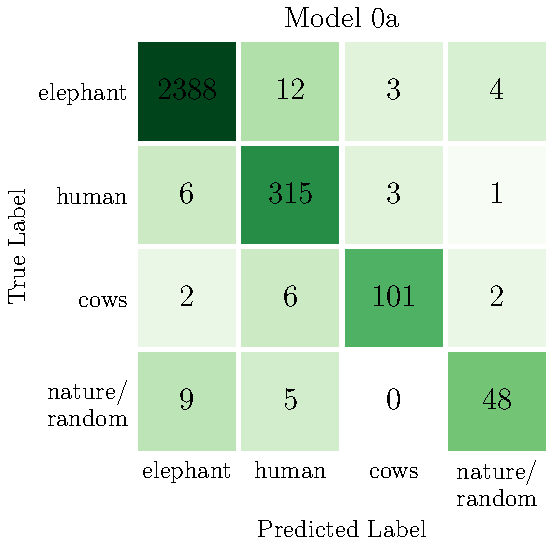
\includegraphics[width=1\linewidth]{0a_cm.pdf} 
    \end{subfigure}
    \begin{subfigure}{0.5\textwidth}
        \centering
        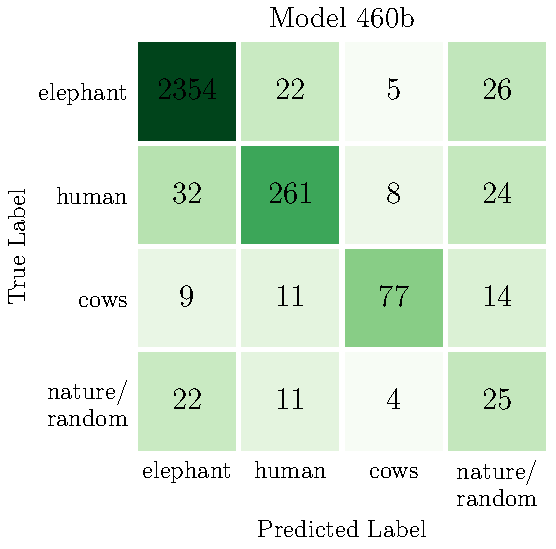
\includegraphics[width=1\linewidth]{460b_cm.pdf}
    \end{subfigure}
    \caption{Confusion matrices of \textit{0a} model (left) and \textit{460b} model (right).}
    \label{double_cm}
\end{figure}
\newpage

\subsection{ Comparison with Edge Impulse models}

We wanted to take our 6 models and compare them against 6 Edge Impulse models that were created by using the same hyperparameters.
However, at the time of writing Edge Impulse supported only model training on images of same dimensions.
Images with different dimensions could either be cropped or scaled to fit 1:1 ratio.
Using the same hyperparameters in Edge Impulse Studio, that were used in our models, would always create a models with a smaller number of parameters.
Smaller image creates a smaller network when compared to a bigger image, given that the rest of architecture does not change.
That meant that we could not make a direct comparison between our models and models trained in Edge Impulse Studio.
We also could not perform random search of hyperparameters in Edge Impulse Studio, as this feature was not fully supported at the time of writing this thesis.

We decided to train a few differently sized models, using the same general CNN architecture as before, but with some minor changes in hyperparameter values.
We also trained a few models with Transfer Learning technique.
Edge Impulse offers scaled down versions of pre-trained MobileNetV2\footnotemark NN architecture, which we used.

Tables \ref{ei_models1} and \ref{ei_models2} show properties of Edge Impulse models using CNN architecture and Transfer Learning technique, respectively. 
Table \ref{precision_recall_table_ei} shows calculated precision and recall values of Edge Impulse models using both approaches.
\footnotetext{MobileNetV2 is a efficient, lightweight NN architecture, designed for image recognition tasks, suitable for mobile applications\cite{geron}. MobileNetV2 contains width multiplier hyperparameter, which scales up or down the total number of parameters, thus providing a trade-off between accuracy and computation complexity. Edge Impulse offers three different width multiplier options: 0.35, 0.1 and 0.05.}

We used only two different versions of MobileNetV2, 0.35, and 0.1, as we saw accuracy drop in reduction of width multiplier hyperparameter.
In all cases the pre-trained model was followed by a one or two dense layers, with dropout layers in between.
\clearpage
\begin{table}[!htbp]
    \centering
    \caption{ Properties of Edge Impulse models using CNN architecture.}
    \rowcolors{2}{gray!25}{white}
    \makebox[\textwidth]{%
    \begin{tabular}{llllllllrl}
    \textbf{Model ID} & \rot{FilterNum1} & \rot{FilterNum2} & \rot{FilterNum3} & \rot{DenseSize} & \rot{DropoutRate}  &\rot{FilterSize} & \rot{LearningRate} & \rotatebox{45}{\parbox{2cm}{Number of parameters}} & \rot{Accuracy[\%]}  \\\toprule
        0ei & 72 & 80 & 64 & 72 & 0.4  & 3x4 & 0.0003 & 1,168,804 & 97.7\\
        1ei & 40 & 48 & 32 & 64 & 0.35 & 3x4 & 0.0001 &   503,196 & 97.5\\
        2ei & 40 & 20 & 20 & 48 & 0.25 & 3x4 & 0.0001 &   231,204 & 97.3\\
        3ei & 42 & 44 &  8 & 14 & 0.1  & 3x4 & 0.0003 &    52,272 & 96.6\\\bottomrule
    \end{tabular}}
    \label{ei_models1}
\end{table}
\bigskip
\bigskip
\bigskip
\begin{table}[!htbp]
    \centering
    \caption{ Properties of Edge Impulse models using Transfer Learning technique.}
    \rowcolors{2}{gray!25}{white}
    \makebox[\textwidth]{%
    \begin{tabular}{llllllll}
        \textbf{Model ID} & \rotatebox{45}{\parbox{1cm}{Width \\Multiplier}} & \rot{DenseSize1} & \rot{DenseSize2} & \rot{DropoutRate} & \rot{LearningRate} & \rotatebox{45}{\parbox{2cm}{Number of\\parameters}} & \rot{Accuracy[\%]}  \\\toprule
        0tl & 0.35 & 16 & N/A& 0.1 & 0.0005 & 430,676 & 98.5\\
        1tl & 0.35 & 16 & 16 & 0.1 & 0.0005 & 430,948 & 98.4\\
        2tl & 0.35 & 32 & 32 & 0.1 & 0.0005 & 452,484 & 98.7\\
        3tl & 0.1  & 32 & 32 & 0.1 & 0.0005 & 135,732 & 95.7\\\bottomrule
    \end{tabular}}
    \label{ei_models2}
\end{table}
\bigskip
\bigskip
\bigskip
\begin{table}[!htbp]
    \caption{ Precision and recall metrics of trained Edge Impulse models}
    \rowcolors{2}{gray!25}{white}
    \makebox[\textwidth]{%
    \begin{tabular}{lrrrrrrrr}\toprule
        \textbf{Model ID}               & 0e    & 1e & 2e & 3e & 0tl & 1tl & 2tl & 3tl\\\toprule
        \textbf{Metrics}                &&&&&&&&\\\toprule
        accuracy[\%]                    & \cellcolor{tbyellow} 97.7  
                                        & \cellcolor{tbyellow} 97.5  
                                        & \cellcolor{tbyellow} 97.3  
                                        & \cellcolor{tbyellow} 96.6  
                                        & \cellcolor{tbgreeny} 98.5  
                                        & \cellcolor{tbgreeny} 98.4  
                                        & \cellcolor{tbgreen} 98.7  
                                        & \cellcolor{tbred} 95.7  \\
        number of parameters            & \cellcolor{tbred} 1,169K 
                                        & \cellcolor{tbyellow} 503K 
                                        & \cellcolor{tbgreeny} 231K 
                                        & \cellcolor{tbgreen} 52K 
                                        & \cellcolor{tbyellow} 430K 
                                        & \cellcolor{tbyellow} 431K 
                                        & \cellcolor{tbyellow} 452K 
                                        & \cellcolor{tbgreeny} 136K\\\midrule
        PR of elephant class[\%]        & \cellcolor{tbgreen}  99.69 
                                        & \cellcolor{tbgreeny} 99.53 
                                        & \cellcolor{tbgreeny} 99.42 
                                        & \cellcolor{tbyellow} 99.27 
                                        & \cellcolor{tbyellow} 99.27 
                                        & \cellcolor{tbgreeny} 99.42 
                                        & \cellcolor{tbgreeny} 99.48
                                        & \cellcolor{tbred}    98.65 \\
        PR of human class[\%]           & \cellcolor{tbyellow} 95.05 
                                        & \cellcolor{tbyellow} 95.05 
                                        & \cellcolor{tbyellow} 91.87 
                                        & \cellcolor{tbyellow} 91.52 
                                        & \cellcolor{tbgreen}  97.17 
                                        & \cellcolor{tbyellow} 95.41 
                                        & \cellcolor{tbgreeny} 96.47
                                        & \cellcolor{tbred}    85.16 \\
        PR of cow class[\%]             & \cellcolor{tbyellow} 82.22 
                                        & \cellcolor{tbyellow} 78.89 
                                        & \cellcolor{tbyellow} 82.22 
                                        & \cellcolor{tbyellow} 79.57 
                                        & \cellcolor{tbgreen}  92.22 
                                        & \cellcolor{tbgreeny} 91.01 
                                        & \cellcolor{tbgreen}  92.22 
                                        & \cellcolor{tbred}    75.56 \\
        PR of nature/random class[\%]   & \cellcolor{tbyellow} 63.04 
                                        & \cellcolor{tbyellow} 65.22 
                                        & \cellcolor{tbyellow} 73.91 
                                        & \cellcolor{tbred}    50.0  
                                        & \cellcolor{tbgreeny} 86.96 
                                        & \cellcolor{tbgreeny} 89.13 
                                        & \cellcolor{tbgreen}  91.3 
                                        & \cellcolor{tbyellow} 78.85 \\\midrule
        RE of elephant class[\%]        & \cellcolor{tbgreen}  99.86 
                                        & \cellcolor{tbyellow} 98.91 
                                        & \cellcolor{tbyellow} 98.44 
                                        & \cellcolor{tbyellow} 98.65 
                                        & \cellcolor{tbgreeny} 99.48 
                                        & \cellcolor{tbgreeny} 99.27 
                                        & \cellcolor{tbgreeny} 99.37 
                                        & \cellcolor{tbred}    98.03 \\
        RE of human class[\%]           & \cellcolor{tbyellow} 93.4  
                                        & \cellcolor{tbyellow} 92.44 
                                        & \cellcolor{tbgreeny} 94.2  
                                        & \cellcolor{tbred}    88.4  
                                        & \cellcolor{tbgreeny} 94.5  
                                        & \cellcolor{tbgreen}  95.74 
                                        & \cellcolor{tbgreen}  95.79 
                                        & \cellcolor{tbyellow} 90.26 \\
        RE of cow class[\%]             & \cellcolor{tbyellow} 90.24 
                                        & \cellcolor{tbyellow} 86.59 
                                        & \cellcolor{tbyellow} 84.09 
                                        & \cellcolor{tbyellow} 79.57 
                                        & \cellcolor{tbgreeny} 92.22 
                                        & \cellcolor{tbyellow} 89.01 
                                        & \cellcolor{tbgreen} 94.32 
                                        & \cellcolor{tbred} 67.33 \\
        RE of nature/random class[\%]   & \cellcolor{tbyellow} 87.88 
                                        & \cellcolor{tbyellow} 88.24 
                                        & \cellcolor{tbyellow} 94.44 
                                        & \cellcolor{tbgreeny} 95.83 
                                        & \cellcolor{tbgreeny} 95.24 
                                        & \cellcolor{tbgreen} 97.62 
                                        & \cellcolor{tbgreeny} 95.45 
                                        & \cellcolor{tbyellow} 91.11 \\\bottomrule
    \end{tabular}}
    \label{precision_recall_table_ei}
\end{table}
\clearpage

Some observations:
\begin{itemize}
    \item Models using CNN architecture did not out perform our models in terms of accuracy. Models \textit{2a} and \textit{0b} both had accuracy of 98.04 \%, while none of Edge Impulse models with CNN architecture did not pass 98 \%.
    \item Most of models trained with Transfer Learning technique out performed our models.
    \item Model \textit{2tl} performed exceptionally well, reaching accuracy of 98.7 \%, while having a relatively small number of parameters.
    \item We saw that by decreasing width multiplier we did not benefit much in accuracy as much as we lost in model size. Even increasing the sizes of dense layers did not solve the problem. 
\end{itemize}

https://towardsdatascience.com/bar-chart-race-in-python-with-matplotlib-8e687a5c8a41


\section{ On device performance testing}
Describe setup

To profile execution of our code we first wrote a timer driver based on a Arm's systick timer, however we later decided to use data watch trigger (DWT).
DWT does not use interrupts, therefore it does not introduce overhead of calling interrupt routines like systick timer does.


      how are you timing, 


\subsection{ Comparison of different optimisation options}

0b
----
0s 11295 ms
03 4117  ms
CMSIS-NN 1023 ms
I and D Cache, Flash prefetch and ART 228ms

\begin{figure}[ht]
    \centering
    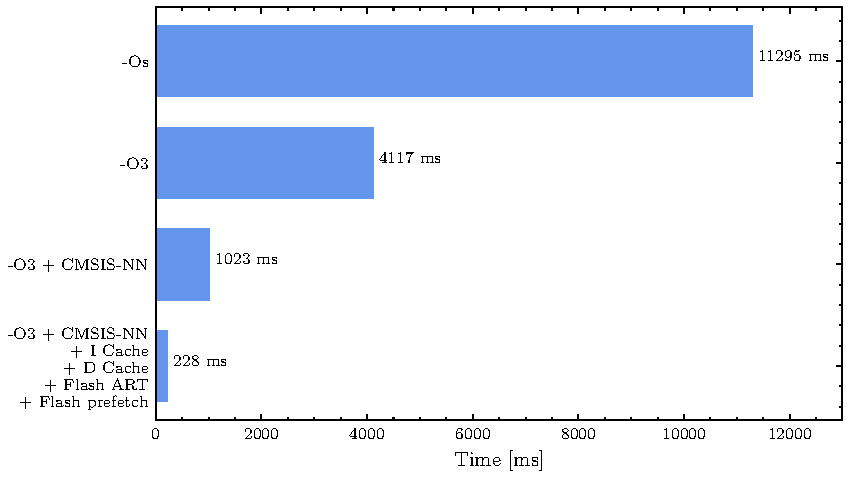
\includegraphics[width=1\linewidth]{opt_comp.pdf}
    \caption{ Speed comparison of different optimizations.}
    \label{opt_comp}
\end{figure}


\subsection{ Comparison of performance of selected models}
    Transfer learning could be interesting here, bigger number of parameters and takes less time.

% Some error below
%\begin{table}
%    \centering
%    \caption{ Second hyperparameter search space}
%    \rowcolors{2}{gray!25}{white}
%    \begin{tabular}{ lrrrrrrrrr}\toprule
%        \textbf{Models}                 &        0a &      2a &      0b &   172b &   338b &   460b &   fast_model\\\toprule
%        \textbf{Metrics}                &&&&&\\\toprule
%        accuracy[\%]                    &     98.18 &   98.04 &   98.04 &  96.80 &  96.28 &   93.4 &    N/A\\
%        number of parameters            &       N/A & 656,797 & 304,216 & 60,672 & 20,290 & 13,114 &    N/A\\ 
%        used flash (in bytes)           &       N/A &  799640 &  445736 & 202424 & 159720 & 152920 & 499592\\ 
%        used ram   (in bytes)           &       N/A &  257032 &  271656 & 260936 &  31704 &  47440 & 198512\\ 
%        time of inference               &       N/A &   403ms &   228ms &  354ms &   51ms &   69ms &    173\\ 
%    \end{tabular}
%    \label{precision_recall_table}
%\end{table}


%mode numparam accu flash ram speed
%0ei 1,168,804 & 97.7 & 1274376 & 5192 & 797
%1ei   503,196 & 97.5 & 606920  & 5192 & 293
%2ei   231,204 & 97.3 & 334120  & 5192 & 150
%3ei    52,272 & 96.6 & 155352  & 5192 & 255
%0tl   430,676 & 98.5 & 695928  & 22024& 108
%1tl   430,948 & 98.4 & 696472  & 22320& 108
%2tl   452,484 & 98.7 & 718104  & 22320& 110
%3tl   135,732 & 95.7 & 346680  & 22448& 73






\section{ Power profiling of an embedded early warning system}

To write this section you need to:
 - wirte uart communication channel for zephyr and your system, has to be simple dont lose time on this.
 - Basic parsing of results and packing them into lora payload
 - Zephyr, put system to sleep and wake it up with pir, turn on fet.
 - Make an image with flir and do inference on it, (subtract mean image, you could test this on real dataset, without subtracted mean)

- [ ] Power consumption test of whole setup, 
      PIR wakes up wisent, 
      wisent turns on stm32f7 and flir, 
      which makes a picture, does inference, reports result and wisent sends the result. 
      Otii image of consumption with marked sections.(shouldnt be hard)

\subsection{ Battery life estimations}
Based on numbers and different scenarios estimate how long would this last with different batteries.
